\documentclass[12pt]{beamer}
\usepackage[latin1]{inputenc}
\usepackage{fancybox}
\usepackage{soul}
\usepackage{wasysym}
\usecolortheme{wolverine}
\usepackage{graphicx}

\title[]{INF5050 - Protocols and routing in internet}
\subtitle[]{Multiprotocol Label Switching (MPLS) / \\
			Generalized Multiprotocol Label Switching (GMPLS) }

\author{Khiem-Kim Ho Xuan -- kkho@ifi.uio.no, \\
		Mattias H�heim Johnsen -- mattiahj@ifi.uio.no}
\date{1. March 2013}


\begin{document}


\begin{frame}
  \titlepage
\end{frame}

\begin{frame}
  \frametitle{Outline}
  \begin{itemize}
  \item Background
  \item MPLS: Fundamentals
  \item MPLS: Terminology
  \item GMPLS
  \item GMPLS: Recovery techniques
  \item Summary
  \item Resources
  
  \end{itemize}
\end{frame}

\begin{frame}
  \frametitle{Background}
  \begin{itemize}
	\item What is MPLS?
		\begin{itemize}
			\item MPLS is a scalable data-carrying mechanism that directs data from one network node to the next based on short path labels rather than network addresses.
            \item Every network packet is assigned at least one label and packet-forwarding decisions are based on them exclusivly, rather than the content of the packets.
            \item Operates somewhere between layer 2 (data link layer) and layer 3 (network layer). Considered a "layer 2.5" protocol.
		\end{itemize}
	
	\item Why MPLS?
		\begin{itemize}
            \item Avoids complex lookups in a routing table.
            \item Create end-to-end circuits using any protocol over any transport medium.
			\item Provide a highly scalable mechanism that was topology driven rather than flow driven.

		\end{itemize}			
	\end{itemize} 

  \bigskip

\end{frame}

\begin{frame}
	\frametitle{Background}
	\begin{itemize}
			\item Load balance traffic to utilize network bandwidth efficiently.
			\item Allow core routers/networking devices to switch packets based on a simplified header.
			\item Remove the complexity and overhead of network managements (Assemble and reassemble IP packets).		
	\end{itemize}
\end{frame}


\begin{frame}
  \frametitle{MPLS was conceived, why?}
  	\begin{itemize}
  		\item The shortest path routing protocols like IS-IS and OSPF
  			\begin{itemize}
  				\item Did not take capacity characteristics into account while
  				making the routing decisions
  				\item The outcome is, segmentation over the network which leads
  				to congestion, while others remain under-utilized.
  			\end{itemize}
  		\item MPLS reduces the complexity and redundancies by adding new network
  		functionalities.
  	\end{itemize}
\end{frame}

\begin{frame}
  \frametitle{MPLS Fundamentals}

  \begin{itemize}
  \item Main idea:
  		\begin{itemize}
  			\item attach a short fixed-length label to packets at the ingress to an MPLS domain
  			\item the labels are used to make the forwarding decisions.
  		\end{itemize}
  	\item MPLS consists of a forwarding and a control plane. Though they are decoupled
  	and independent from each other.
  	\item Supports explicit routed path.
  	\item Provides Quality of Service (QoS) if it is implemented with Diff-Serv and Constraint-based routing.

  \end{itemize}
\end{frame}


\begin{frame}
	\frametitle{Diff-Serv and Constraint-based routing}
		\begin{itemize}
			\item Differentiated Services
				\begin{itemize}
					\item A network architecture for classifying and managing network traffic and provide QoS on modern IP networks.
					\item it is used to provide low-latency to critical network traffic. (Media, VOIP).
				\end{itemize}
			\item Constraint-based routing
				\begin{itemize}
					\item It is a routing technique where resource availability and traffic characterization are taken into account.
				\end{itemize}
		\end{itemize}

\end{frame}

\begin{frame}
	\frametitle{MPLS Fundamentals}
		\begin{figure}[h]
			\begin{center}
				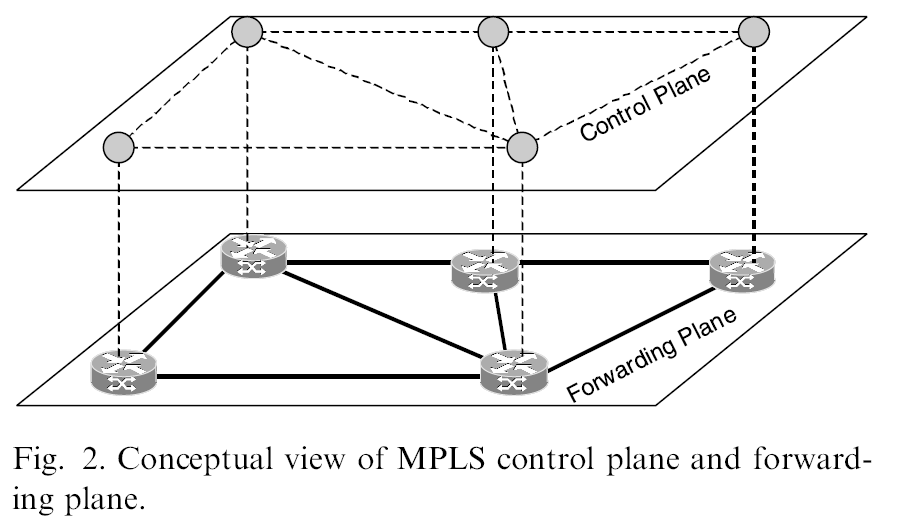
\includegraphics[scale=0.40]{separation.png}
			\end{center}
		\end{figure}
\end{frame}

\begin{frame}
	\frametitle{MPLS Fundamentals: Control Plane}
	
\end{frame}

\begin{frame}
	\frametitle{MPLS Fundamentals: Forwarding Plane}
	
\end{frame}

\begin{frame}
	\frametitle{MPLS architecture}
	
\end{frame}


\begin{frame}
	\frametitle{MPLS: Terminology}
	
	\begin{itemize}
		\item FEC (Forwarding Equivalence Class)
			\begin{itemize}
				\item Group of IP packets which are forwarded in the same manner (e.g. over the same path, with the same priority and the same label)
			\end{itemize}
			
		\item Label
			\begin{itemize}
				\item Short fixed length identifier which is used to identify a FEC
			\end{itemize}						
			
		\item Label Swapping
			\begin{itemize}
				\item Looking up the oncoming label to determine the outgoing label, encapsulation and port
			\end{itemize}
			
		\item Label switched path (LSP)
			\begin{itemize}
				\item Path through one or more LSR for a particular FEC
			\end{itemize}
		\item Label switching router (LSR)
			\begin{itemize}
				\item an MPLS capable router
			\end{itemize}
			
			
	\end{itemize}

\end{frame}

\begin{frame}
	\frametitle{FEC}

	Advantages?	
	\begin{itemize}
		\item 
	\end{itemize}
\end{frame}

\begin{frame}
	\frametitle{What is a Label?}
	
	\begin{itemize}
		\item an extra layer that "sits" between L2 and L3 layer
		known as header 2.5 (or "shim")
		\item don't need to lookup at the routing table, you use the label information
		to find the next hop
		\item creates a VPN rather than public networks
		\item isolates other traffics running on the network

	\end{itemize}

		\begin{figure}[h]
			\begin{center}
				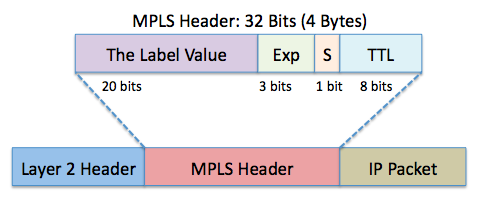
\includegraphics[scale=0.40]{header_mpls.png}
			\end{center}
		\end{figure}	
	
	
\end{frame}

\begin{frame}
	\frametitle{What is a Label?}
	Header information
	\begin{itemize}
		\item \bf{Label value: }the label itself for lookup in the MPLS forwarding table
		\item \bf{EXP field: }gives Diffserv support on the MPLS network and carry the IP precedence value from the IP packet.
		\item \bf{Stack bit: }Indicates the bottom of the MPLS header stack has been reached.
		\item \bf{Time-To-Live: }prevents loop and path tracing in the MPLS network. This value decrements with each hop and packet discards occur at a zero value.
	\end{itemize}		
	
\end{frame}


\begin{frame}
	\frametitle{Label distribution in MPLS and how LSP works}
\begin{figure}
	%This is how you would give a good animation
    \includegraphics<1>[scale=0.5]{animations/routeInit.png}
    \includegraphics<2>[scale=0.5]{animations/routereq1.png}
    \includegraphics<3>[scale=0.5]{animations/routereq2.png}
    \includegraphics<4>[scale=0.5]{animations/labeltable1.png}
    \includegraphics<5>[scale=0.5]{animations/labeltable2.png}
    \includegraphics<6>[scale=0.5]{animations/labeltable3.png}
    \includegraphics<7>[scale=0.5]{animations/labeltable4.png}
    \includegraphics<8>[scale=0.4]{animations/labeltable5.png}
    \includegraphics<9>[scale=0.4]{animations/path1.png}
    \includegraphics<10>[scale=0.4]{animations/path2.png}
    \includegraphics<11>[scale=0.4]{animations/path3.png}
    \caption{\only<1>{This is the initial phase}
    \only<2>{Ingress node makes a request to the nearest node for a given destination address}
    \only<3>{Route the message to the destination node}
    \only<4>	{A label table is initialized with information that when it receives the given label id, it is for this router 47.1}
    \only<5>{Map its label id to the router that sent request}
    \only<6>{The router that receives the mapping data, adds it to its forwarding table and generates a "in" label}
    \only<7>{When finished, the egress node sends the mapping date of which label
    will be added }    
    \only<8>{When it has reached the Ingress node, it will map the given label for the
    given destination IP}
    \only<9>{Send message/packet to 47.1, the Ingress node makes a routing lookup and
   assigns the given label for the destination}
    \only<10>{When forwarded, you add label onto the packet, when it arrives to 
    a node, it checks the label and replaces it to another one and forwards it}
    \only<11>{When reached to the egress node, it will then strip out the label and deliver to the specific destination}
    
    }

\end{figure}  	
	

\end{frame}


\begin{frame}
\frametitle{Disadvantages of MPLS}
	MPLS has performance issues in the network:
	\begin{itemize}
		\item constraint-based routing
			\begin{itemize}
				\item Problem with computation of paths for LSPs subject to various types of constraints.
				\item NP-complete problem
			\end{itemize}
		\item traffic partitioning and assignment
			\begin{itemize}
				\item This problem deals with the optimal partitioning and assignment of traffic to parallel LSPs between pairs of MPLS ingress and egress nodes.
			\end{itemize}					
		\item Low visibility and lack of access into the MPLS cloud. How to monitor that your carrier is delivering the correct performance? 
            \begin{itemize}
                \item Trace-route and ping no longer an option.
                \item Probes are costly and difficult to maintain.
            \end{itemize}
        \item restoration
		\begin{itemize}
			\item many proposals for restoration in ATM might be applicable to MPLS.
		\end{itemize}				
	\end{itemize}
\end{frame}

\begin{frame}
  \frametitle{GMPLS}

  \begin{itemize}
  \item What is GMPLS?
  	\begin{itemize}
  		\item  a protocol suite extending MPLS to manage further classes of interfaces and switching technologies other than packet interfaces and switching, such as time division multiplex, layer-2 switch, wavelength switch and fiber-switch.
  	\end{itemize}
  \end{itemize}
\end{frame}

\begin{frame}
	\frametitle{GMPLS}
	\begin{itemize}
	

	  		\item GMPLS is an extended form of MPLS and some of these improvements are:
			\begin{itemize}
				\item RSVP-TE
				\item OSPF and IS-IS
				\item New link-management protocol
				\item Bi-directional LSP setup
					\begin{itemize}
						\item Reduce latency
						\item Less control overhead
						\item Route selection is simpler
						\item Cleaner interface
					\end{itemize}									
			\item MPLS emphasizes the seperation of control plane and network plane
			\item GMPLS extends this seperation and allows the control plane to be physically diverse from the associated data plane
				
			\end{itemize}		
				\end{itemize}
\end{frame}

\begin{frame}
  \frametitle{GMPLS: Hierarchial LSP}

  \begin{itemize}
  \item 
    %\pause
  \item 
  \end{itemize}
\end{frame}




\begin{frame}
  \frametitle{Summary}
  \begin{itemize}
  \item MPLS
    %\pause
  \item GMPLS
  \end{itemize}
\end{frame}

\begin{frame}
  \frametitle{Resources}
  \begin{itemize}
  \item Generalized Multiprotocol Label Switching: An Overview of Signaling Enhancements and Recovery Techniques
IEEE Communication Magazine, July 2001.
A. Banerjee et. al. 
  \item Internet Traffic Engineering Using Multi-Protocol Label Switching (MPLS).
Computer Networks 40, Elsevier, 2002
D.O. Awduche and B. Jabbari. 
  \end{itemize}
\end{frame}

\end{document}
